\documentclass[conference]{IEEEtran}
\usepackage[T1]{fontenc}
\usepackage[utf8]{inputenc}
\usepackage{lmodern}
\usepackage{cite}
\usepackage{amsmath,amssymb}
\usepackage{graphicx}
\usepackage{booktabs}
\usepackage{multirow}
\usepackage{tikz}
\usepackage{hyperref}
\usepackage{xcolor}
\usetikzlibrary{arrows.meta,positioning,fit,calc,shapes.geometric,backgrounds}
\hypersetup{hidelinks}

\title{Toward a Standardizable Compute Intelligence Graph (CIG):\\
A Provider-Agnostic Reference Model for Infrastructure Intelligence and Agent-Grounded Operations}

\author{\IEEEauthorblockN{Anonymous Submission}}

\begin{document}
\maketitle

\begin{abstract}
Infrastructure operations remain fragmented across clouds, on-premise environments, orchestration frameworks, observability stacks, and policy systems. Although graph-based representations, knowledge engineering, digital twins, and recent agentic AIOps frameworks each address part of this problem, current solutions remain siloed by domain, execution plane, or vendor. This paper proposes the Compute Intelligence Graph (CIG), a provider-agnostic reference model that unifies infrastructure resources, dependencies, policies, observations, actions, and provenance in a single graph-centered control abstraction. The contribution is not a claim of a new primitive, but a formalization of how existing graph, agent, and infrastructure patterns can be composed into a standardizable architecture. We review the current state of the art in infrastructure graphs, cloud knowledge modeling, digital twins, infrastructure-as-code knowledge support, and agentic operations; identify the interoperability gap between discovery, reasoning, and actuation; and present CIG as a layered model with explicit standardization surfaces for schema, query, policy, action, and provenance. We argue that CIG can serve as a reference architecture for scalable, self-hosted, and multi-environment infrastructure intelligence systems, and outline an evaluation agenda for interoperability, governance, and adoption.
\end{abstract}

\begin{IEEEkeywords}
Infrastructure intelligence, knowledge graph, property graph, digital twin, AIOps, agent systems, multi-cloud, infrastructure-as-code, standardization.
\end{IEEEkeywords}

\section{Introduction}
Modern infrastructure operations are no longer bounded to a single control plane. Production systems span public clouds, private clusters, edge resources, identity systems, databases, and policy engines. The resulting operational reality is fragmented: topology is discovered in one tool, cost in another, security posture in another, infrastructure-as-code (IaC) in another, and increasingly, conversational or agentic automation in yet another. This fragmentation is structural rather than incidental.

Recent work shows that graph-based representations can capture rich dependencies in cloud and infrastructure settings, enabling optimization, security analysis, and semantic integration \cite{khan2024cost,li2024infrastructuredt,schoberl2024certgraph,cartography2026}. In parallel, agentic AIOps and AI-agent infrastructure research emphasize that next-generation operational systems require explicit mechanisms for attribution, policy shaping, safe action, and end-to-end task orchestration \cite{zota2025agentic,chen2025aiopslab,hadfield2025infraagents}. Yet these lines of work remain only loosely connected.

This paper argues for a provider-agnostic intermediate model: the \emph{Compute Intelligence Graph} (CIG). CIG is defined as a graph-centered abstraction that represents infrastructure entities, relationships, policies, observations, available actions, and provenance in a unified control model. The proposed contribution is threefold:
\begin{enumerate}
    \item a structured synthesis of the state of the art across infrastructure graphs, digital twins, IaC knowledge support, and agentic operations;
    \item a reference model for integrating discovery, reasoning, and actuation over heterogeneous environments; and
    \item a standardization path based on explicit surfaces for graph schema, query, policy, action, and provenance.
\end{enumerate}

The paper is intentionally agnostic with respect to cloud provider, orchestrator, graph database, or model provider. Its goal is to describe what would be required for CIG to evolve from an architectural pattern into a reusable standard.

\section{State of the Art}
\subsection{Knowledge Graphs and Property Graphs}
Knowledge graphs provide a mature foundation for integrating heterogeneous, evolving, and semantically rich data \cite{hogan2021kg}. In practice, both RDF-based and property-graph-based models are relevant. RDF remains central for interoperability and ontology alignment \cite{w3c2014rdf}, while the publication of ISO/IEC 39075:2024 established GQL as the first ISO standard for property-graph query and data manipulation \cite{iso2024gql}. For infrastructure intelligence, property graphs are attractive because they naturally support typed nodes and relationships, path traversals, and incremental enrichment of operational metadata.

\subsection{Infrastructure Graphs and Cloud Discovery}
Open-source systems such as Cartography demonstrate the practical value of consolidating infrastructure assets and relationships in Neo4j-backed graph views, particularly for dependency analysis and security exploration \cite{cartography2026}. Meanwhile, research has extended graph approaches to cloud cost optimization, showing that resource placement, utilization, cost, performance, and availability can be modeled as a graph-constrained optimization problem \cite{khan2024cost}. These efforts validate the graph as a useful representation, but they typically optimize a single concern (e.g., cost or security) rather than providing a general control abstraction.

\subsection{Ontology-Driven Infrastructure and Digital Twins}
Ontology-based representations have long been proposed for cloud service discovery and interoperability \cite{youssef2013cocoon}. More recently, infrastructure digital twins have adopted graph-represented ontologies to model multi-scale, multi-object, and cross-scenario infrastructure systems \cite{li2024infrastructuredt}. Domain-agnostic digital twin graph construction has also been studied as a way to automate twin generation from raw data rather than relying exclusively on handcrafted expert models \cite{du2023dtg}. These works are especially relevant because they elevate graph representations from static inventory to live operational models.

\subsection{Knowledge Support for Infrastructure-as-Code}
IaC remains the dominant abstraction for declarative deployment, but it is not itself a semantic integration model. Recent work on knowledge-guided IaC development shows that ontologies can support auto-completion, error detection, and matchmaking across deployment artifacts, especially when aligned to open standards such as TOSCA \cite{vasileiou2025iac}. Related modeling efforts such as DOML aim to reduce the expertise burden of multiple IaC dialects through higher-level abstractions \cite{doml2023}. These contributions suggest that knowledge layers can complement IaC, but the broader question of runtime graph alignment across actual deployed resources remains open.

\subsection{Agentic AIOps and Agent Infrastructure}
The operational role of AI agents is receiving increasing attention. Agentic AIOps frameworks argue for autonomous diagnosis, prevention, and resolution across infrastructure, middleware, data, and applications \cite{zota2025agentic}. AIOpsLab strengthens this line by providing an evaluation framework for end-to-end and multitask AIOps agents in microservice cloud environments \cite{chen2025aiopslab}. At a more foundational level, \emph{Infrastructure for AI Agents} argues that agent ecosystems require explicit infrastructure for identity attribution, interaction shaping, and remediation of harmful actions \cite{hadfield2025infraagents}. However, these works do not yet converge on a standard operational substrate that grounds agents in heterogeneous infrastructure reality.

\subsection{Graph-Grounded AI over Infrastructure}
A particularly relevant emerging direction is the use of graph-grounded retrieval and reasoning over cloud configuration and infrastructure data. RIG-RAG proposes a typed knowledge graph and GraphRAG-style inference pipeline for natural-language reasoning about cloud infrastructure \cite{rigrag2025}. Likewise, recent work on ontology-driven NLP for cloud resource queries reinforces the need for semantic grounding rather than keyword search \cite{sunkara2025ontology}. These approaches are directionally aligned with CIG, but are still largely solution-specific rather than framed as an interoperable architectural standard.

\subsection{Gap Analysis}
The literature strongly suggests that graph representations, ontology support, digital twin thinking, and agentic operations are converging. Yet the state of the art still exhibits five recurring gaps:
\begin{enumerate}
    \item \textbf{Graphs are usually single-purpose.} Most systems optimize cost, security, discovery, or querying, but not a unified operational plane.
    \item \textbf{Agent frameworks are under-grounded.} Agents often reason over logs, prompts, or tool lists rather than a durable infrastructure graph.
    \item \textbf{Discovery and actuation are disconnected.} Inventory systems and IaC systems rarely share a live, typed semantic substrate.
    \item \textbf{Provider-specific abstractions dominate.} Many tools remain tied to a cloud vendor, a control plane, or a single execution environment.
    \item \textbf{Standardization is incomplete.} We now have GQL for property-graph operations \cite{iso2024gql}, but not a comparable standard for infrastructure intelligence objects, actions, or provenance.
\end{enumerate}

\section{Design Goals}
To be viable as a standardizable model rather than a vendor-specific product architecture, CIG should satisfy the following design goals.

\subsection{Provider Agnosticism}
The model must not depend on a single cloud, orchestration stack, or deployment target. It should be applicable to cloud, on-premise, edge, and hybrid settings.

\subsection{Bidirectional Semantics}
The model must support both \emph{reflection} (discovering and querying the world as it is) and \emph{projection} (declaring, recommending, or executing changes to that world).

\subsection{Agent Grounding}
Agent reasoning must be grounded in typed graph entities, policies, and evidence, rather than prompt-only heuristics.

\subsection{Policy and Provenance by Construction}
Operational systems require not only topology but also permissions, action constraints, authorship, and evidence trails.

\subsection{Incremental Adoption}
The model should support adoption as an overlay on existing systems (e.g., Cartography, Terraform, Kubernetes, observability stacks), without requiring a greenfield rewrite.

\section{The Compute Intelligence Graph Reference Model}
\subsection{Definition}
We define the Compute Intelligence Graph (CIG) as follows:
\begin{quote}
\emph{A provider-agnostic, graph-centered control abstraction that represents infrastructure resources, services, identities, policies, observations, actions, and provenance as a unified and queryable operational graph for both human and agent-driven reasoning.}
\end{quote}

The emphasis is on \emph{operational graph} rather than only a data graph. CIG is not merely an inventory or digital twin; it is the substrate on which discovery, reasoning, governance, and actuation meet.

\subsection{Layered Architecture}
Fig.~\ref{fig:layers} presents the layered model.

\begin{figure}[t]
\centering
\resizebox{0.98\columnwidth}{!}{%
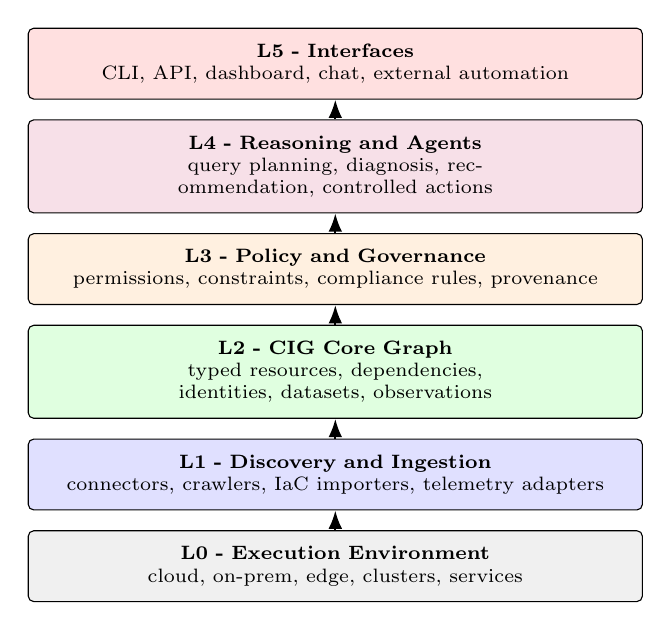
\begin{tikzpicture}[
  >=Latex,
  every node/.style={font=\scriptsize},
  layer/.style={draw, rounded corners=2pt, align=center, minimum height=8mm, text width=7.4cm, inner sep=2mm, fill=#1!12}
]
\node[layer=gray] (l0) {\textbf{L0 - Execution Environment}\\cloud, on-prem, edge, clusters, services};
\node[layer=blue, above=2.5mm of l0] (l1) {\textbf{L1 - Discovery and Ingestion}\\connectors, crawlers, IaC importers, telemetry adapters};
\node[layer=green, above=2.5mm of l1] (l2) {\textbf{L2 - CIG Core Graph}\\typed resources, dependencies, identities, datasets, observations};
\node[layer=orange, above=2.5mm of l2] (l3) {\textbf{L3 - Policy and Governance}\\permissions, constraints, compliance rules, provenance};
\node[layer=purple, above=2.5mm of l3] (l4) {\textbf{L4 - Reasoning and Agents}\\query planning, diagnosis, recommendation, controlled actions};
\node[layer=red, above=2.5mm of l4] (l5) {\textbf{L5 - Interfaces}\\CLI, API, dashboard, chat, external automation};
\foreach \a/\b in {l0/l1,l1/l2,l2/l3,l3/l4,l4/l5}{\draw[->, thick] (\a.north) -- (\b.south);} 
\end{tikzpicture}%
}
\caption{Layered reference architecture for CIG. The model separates environment discovery, graph construction, governance, reasoning, and interface concerns.}
\label{fig:layers}
\end{figure}

\subsection{Core Entity Classes}
CIG should define a minimal portable ontology or property-graph schema with the following first-class entity classes:
\begin{itemize}
    \item \textbf{Environment}: cloud account, cluster, host, region, tenant.
    \item \textbf{Resource}: compute instance, function, bucket, database, queue, network, secret, service.
    \item \textbf{Identity}: user, role, service account, workload identity, machine identity.
    \item \textbf{Policy}: access rule, compliance rule, placement rule, operational guardrail.
    \item \textbf{Observation}: metric, event, alert, trace, change event.
    \item \textbf{Action}: supported mutation or workflow, with preconditions and expected effects.
    \item \textbf{Provenance}: source, timestamp, tool, confidence, evidence, actor.
\end{itemize}

Rather than forcing a single ontology language, the model can be implemented as a property graph with optional semantic bindings to RDF/OWL for interoperability.

\subsection{Reference Relationships}
The graph must support at least the following relationships:
\begin{itemize}
    \item \texttt{DEPENDS\_ON}
    \item \texttt{RUNS\_ON}
    \item \texttt{CONNECTS\_TO}
    \item \texttt{USES\_ID}
    \item \texttt{EMITS}
    \item \texttt{CONSTRAINED\_BY}
    \item \texttt{ACTION\_ON}
    \item \texttt{DERIVES}
    \item \texttt{OBS\_BY}
    \item \texttt{ATTESTS}
\end{itemize}

This relationship set intentionally spans topology, semantics, policy, and evidence. Fig.~\ref{fig:schema} sketches a portable subgraph.

\begin{figure}[t]
\centering
\resizebox{0.94\columnwidth}{!}{%
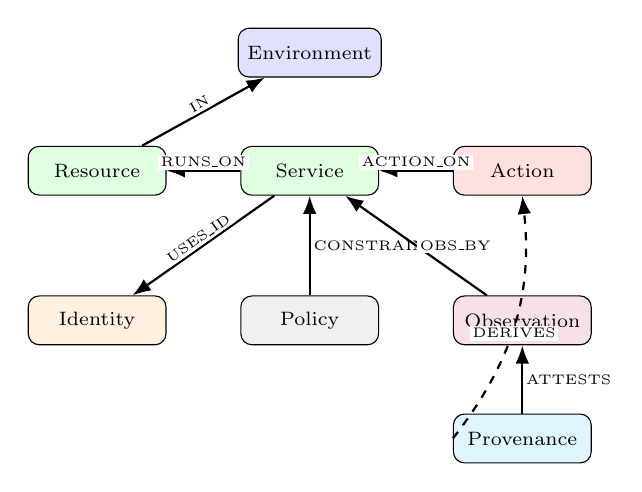
\begin{tikzpicture}[
  >=Latex,
  every node/.style={font=\scriptsize},
  box/.style={draw, rounded corners, minimum width=1.75cm, minimum height=0.62cm, align=center, fill=#1!12},
  rel/.style={->, thick},
  lab/.style={font=\tiny, fill=white, inner sep=1pt}
]
\node[box=blue]   (env)  at (0, 1.9)  {Environment};
\node[box=green]  (res)  at (-2.7, 0.4) {Resource};
\node[box=green]  (svc)  at (0, 0.4)  {Service};
\node[box=red]    (act)  at (2.7, 0.4)  {Action};
\node[box=orange] (id)   at (-2.7,-1.5) {Identity};
\node[box=gray]   (pol)  at (0,-1.5)  {Policy};
\node[box=purple] (obs)  at (2.7,-1.5)  {Observation};
\node[box=cyan]   (prov) at (2.7,-3.0) {Provenance};

\draw[rel] (svc) -- node[lab, above] {RUNS\_ON} (res);
\draw[rel] (res) -- node[lab, sloped, above] {IN} (env);
\draw[rel] (svc) -- node[lab, sloped, above] {USES\_ID} (id);
\draw[rel] (pol) -- node[lab, right] {CONSTRAINS} (svc);
\draw[rel] (obs) -- node[lab, right] {OBS\_BY} (svc);
\draw[rel] (act) -- node[lab, above] {ACTION\_ON} (svc);
\draw[rel] (prov) -- node[lab, right] {ATTESTS} (obs);
\draw[rel, dashed] (prov.west) to[bend right=22] node[lab, below] {DERIVES} (act.south);
\end{tikzpicture}%
}
\caption{Minimal portable subgraph in the CIG model. A standard should specify the mandatory node classes, relationship vocabulary, and required provenance fields.}
\label{fig:schema}
\end{figure}

\subsection{Control Loops}
CIG unifies three control loops that are often separate in practice:
\begin{enumerate}
    \item \textbf{Reflective loop}: discover resources and update graph state.
    \item \textbf{Analytical loop}: query, diagnose, compare, or optimize over graph state.
    \item \textbf{Actuation loop}: execute guarded actions and re-ingest resulting state transitions.
\end{enumerate}

Fig.~\ref{fig:loop} shows the agent-grounded control loop.

\begin{figure}[t]
\centering
\resizebox{0.96\columnwidth}{!}{%
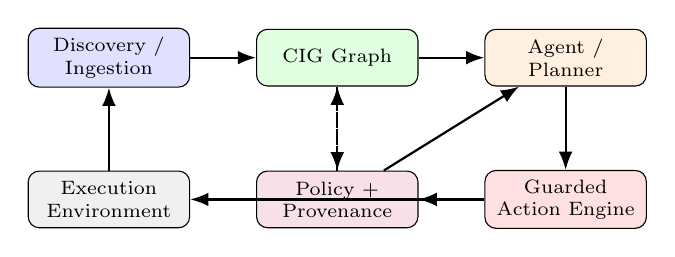
\begin{tikzpicture}[
  >=Latex,
  comp/.style={draw, rounded corners, minimum width=2.05cm, minimum height=0.72cm, align=center, fill=#1!12},
  arr/.style={->, thick},
  every node/.style={font=\scriptsize}
]
\node[comp=blue] (disc) at (0,0) {Discovery /\\Ingestion};
\node[comp=green] (graph) at (2.9,0) {CIG Graph};
\node[comp=orange] (agent) at (5.8,0) {Agent /\\Planner};
\node[comp=gray] (env) at (0,-1.8) {Execution\\Environment};
\node[comp=purple] (policy) at (2.9,-1.8) {Policy +\\Provenance};
\node[comp=red] (act) at (5.8,-1.8) {Guarded\\Action Engine};

\draw[arr] (env) -- (disc);
\draw[arr] (disc) -- (graph);
\draw[arr] (graph) -- (agent);
\draw[arr] (policy) -- (agent);
\draw[arr] (agent) -- (act);
\draw[arr] (act) -- (env);
\draw[arr] (act) -- (policy);
\draw[arr, dashed] (graph) -- (policy);
\draw[arr, dashed] (policy) -- (graph);
\end{tikzpicture}%
}
\caption{Agent-grounded operational loop. Agents consume graph state and policy context; actions update the environment and emit provenance back into the graph.}
\label{fig:loop}
\end{figure}

\section{Standardization Surfaces}
If CIG is to become more than a system architecture, it needs explicit standardization surfaces. We propose five.

\subsection{Graph Schema Surface}
A standard should define a portable core schema: mandatory node kinds, mandatory relationships, required metadata, and cardinality constraints. This is analogous to how RDF and OWL define graph data and semantics, but adapted to operational infrastructure concerns \cite{w3c2014rdf,hogan2021kg}. The graph schema surface should remain small enough for broad adoption, with profiles for cloud, Kubernetes, data, and policy domains.

\subsection{Query Surface}
CIG should not invent a new graph query language. Instead, it should adopt the emerging property-graph standard ecosystem around GQL and remain mappable to Cypher-like implementations \cite{iso2024gql}. Standardization should focus on portable named queries, graph views, and semantic query intents rather than syntax reinvention.

\subsection{Policy Surface}
A CIG-compliant system should expose machine-readable constraints over graph entities and actions. At minimum, this includes access control constraints, change-approval requirements, compliance tags, and safety guards for agent actions. This aligns with the need for interaction shaping and remediation infrastructure in agent ecosystems \cite{hadfield2025infraagents}.

\subsection{Action Surface}
The action surface is what distinguishes CIG from a passive graph. A standard should define how actions are declared, parameterized, authorized, simulated, executed, and audited. This could resemble a typed tool contract, where each action specifies:
\begin{itemize}
    \item target entity classes,
    \item preconditions,
    \item required roles or approvals,
    \item expected state transition,
    \item rollback or compensation semantics, and
    \item required provenance outputs.
\end{itemize}

\subsection{Provenance Surface}
Operational trust depends on evidence. Provenance must be first-class: who discovered an entity, when, from which source, with what confidence, under what authorization, and whether an observation or action has been superseded. This is crucial in certification and compliance-oriented graph systems such as CertGraph \cite{schoberl2024certgraph}.

\begin{figure}[t]
\centering
\resizebox{0.92\columnwidth}{!}{%
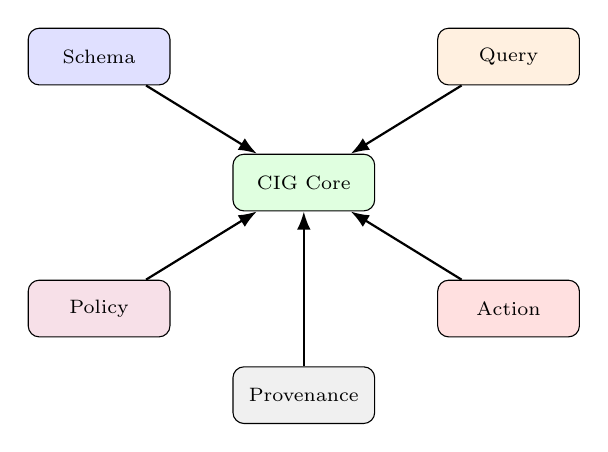
\begin{tikzpicture}[
  >=Latex,
  surf/.style={draw, rounded corners, minimum width=1.8cm, minimum height=0.72cm, align=center, fill=#1!12},
  arr/.style={->, thick},
  every node/.style={font=\scriptsize}
]
\node[surf=green] (core) at (0,0) {CIG Core};
\node[surf=blue] (schema) at (-2.6,1.6) {Schema};
\node[surf=orange] (query) at (2.6,1.6) {Query};
\node[surf=purple] (policy) at (-2.6,-1.6) {Policy};
\node[surf=red] (action) at (2.6,-1.6) {Action};
\node[surf=gray] (prov) at (0,-2.7) {Provenance};

\draw[arr] (schema) -- (core);
\draw[arr] (query) -- (core);
\draw[arr] (policy) -- (core);
\draw[arr] (action) -- (core);
\draw[arr] (prov) -- (core);
\end{tikzpicture}%
}
\caption{Five proposed standardization surfaces for CIG. A successful standard effort should isolate and stabilize these interfaces rather than over-specifying storage or implementation internals.}
\label{fig:surfaces}
\end{figure}

\section{Why CIG Is Provider-Agnostic}
CIG is intentionally not defined by its deployment substrate. The same model can describe AWS resources, on-premise machines, Kubernetes objects, or edge services if they are mapped into the shared graph vocabulary. The provider-specific logic belongs in \emph{connectors} and \emph{ingestion adapters}, not in the core abstraction.

This separation also makes CIG compatible with multiple implementation strategies:
\begin{itemize}
    \item discovery based on Cartography-like crawlers \cite{cartography2026},
    \item IaC ingestion from Terraform/TOSCA/DOML-like models \cite{vasileiou2025iac,doml2023},
    \item observability ingestion from metrics, logs, and traces,
    \item graph storage in Neo4j, JanusGraph, NebulaGraph, or other GQL-compatible or adapter-backed systems,
    \item agent layers implemented with different LLM orchestration stacks.
\end{itemize}

In that sense, CIG is best understood as a \emph{control abstraction and interoperability contract}, not as a specific product.

\section{Research Agenda and Evaluation}
A credible path to standardization requires an evaluation agenda beyond conceptual appeal.

\subsection{Interoperability Benchmarks}
The first research track should evaluate whether different providers and tools can map their entities into the same CIG core without severe semantic loss. This includes cross-cloud resources, Kubernetes objects, identities, and policy objects.

\subsection{Agent Grounding Benchmarks}
Drawing from AIOpsLab \cite{chen2025aiopslab}, one can benchmark whether graph-grounded agents outperform prompt-only agents on infrastructure diagnosis, planning, and change execution. RIG-RAG-style pipelines are an important reference point here \cite{rigrag2025}.

\subsection{Governance and Safety Benchmarks}
A key differentiator for CIG is safe actuation. Evaluation should include not only accuracy of answers and plans, but also policy compliance, rate of unsafe actions prevented, audit completeness, and reversibility of changes.

\subsection{Scalability}
The graph must support large and dynamic environments. Research questions include incremental ingestion, graph compaction, temporal views, partitioning, and federated queries across multiple graph domains. This should be studied as an operational systems problem, not only as a database throughput problem.

\section{Discussion}
The most important claim of this paper is deliberately modest: CIG does not introduce a wholly new computational primitive. Graphs, ontologies, digital twins, IaC abstractions, and agentic operations already exist. The novelty lies in proposing a disciplined way to bind them together into a provider-agnostic standard model.

This also explains the main risk. CIG could easily collapse into an over-scoped “platform for everything.” To avoid that, a future standard effort should remain narrowly focused on the interoperability contract: \emph{what} must be represented, queried, constrained, acted upon, and attested --- not \emph{how} every implementation must store or compute it.

In practice, early adoption is most likely to succeed in incremental deployments: e.g., a Cartography-derived discovery layer writing into a portable graph core, or an IaC-centric workflow augmented with CIG policy and provenance layers. Such an adoption path mirrors how standards typically emerge: first as shared interfaces between already useful components.

\section{Conclusion}
The current literature already validates the building blocks behind CIG: graph-based infrastructure representations, ontology-driven integration, digital twin approaches, knowledge support for IaC, and agentic AIOps. What remains missing is a shared reference model that connects discovery, reasoning, policy, and actuation in a portable way.

This paper proposed the Compute Intelligence Graph as that missing model. We presented CIG as a provider-agnostic, graph-centered operational abstraction; identified the standardization surfaces required for broader adoption; and outlined a research agenda for interoperability, grounding, governance, and scale. If successful, CIG would not compete with existing graph engines, IaC tools, or agent frameworks. Instead, it would provide the missing coordination layer among them.

\section*{Acknowledgment}
This manuscript is a conceptual research proposal intended to support open standardization discussion. It does not claim an existing de jure standardization process.

\bibliographystyle{IEEEtran}
\bibliography{cig_standard}

\end{document}
